\fbox{
\begin{minipage}{0.45\textwidth}

\minisec{Hick-Hyman}
Reaktionszeit $RT = a + b \log_2 ( n + 1 )$\\
a,b konstante, n: Auswahlmöglichkeiten\\
Relevant in Menüs, bei gelernten Einträgen (Unbekannte Einträge: lineare Suchzeit)

\begin{minipage}{0.5\textwidth}
\minisec{Fitts}
$Zeit = a + b \cdot ID$ \\
Fitts: $ID= \log_2(\frac{2A}{W})$\\
MacKenzie: $ID =\cdot \log_2(\frac{D}{W}+1)$ \\
Accot: ID = $\log_2(\sqrt{(\frac{D}{W})^2+\mu(\frac{D}{H})^2}+1) $ 
\end{minipage}
\begin{minipage}{0.4\textwidth}
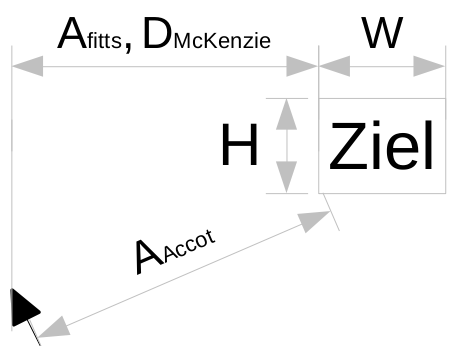
\includegraphics[width=\textwidth]{Fitts}
\end{minipage}

=> Over-/Undershooting: Verfehlen des Zieles, Korrektur nötig\\
Konkurrenz der GUI-Elemente (kleine Ausgabe)\\
stärkere Abweichung für kleine Ziele

Unterstützung: \tab
\begin{minipage}{0.6\textwidth}
\begin{itemize}
\item Vergrößern Ziel/Zeiger
\item Cursor zum Ziel/ Ziel zum Cursor bewegen
\end{itemize}
\end{minipage}

=> evtl. irritierend, ungewollte Auswahl


\end{minipage}
}			